\documentclass[11pt , conference]{IEEEtran}
\usepackage{amsfonts}
\usepackage{booktabs}
\usepackage{siunitx}
\usepackage{cellspace}%
\usepackage{booktabs}
\usepackage{makecell}
\setcellgapes{3pt}
\usepackage{amsmath}
\usepackage{caption}
\usepackage{array}
\newcommand\tab[1][0.5cm]{\hspace*{#1}}
\newcommand{\tsone}{\fontencoding{TS1}\selectfont}
\usepackage{chngcntr}
\usepackage{graphicx}


\usepackage{graphicx}
\usepackage{mathtools}
\usepackage{multirow}
\usepackage[justification=centering]{caption}
\usepackage{amsmath}
\usepackage{float}
\usepackage[table]{xcolor}
\usepackage[linesnumbered,ruled,vlined]{algorithm2e}
\usepackage{algpseudocode}
\usepackage{cite}
\usepackage{subcaption}
\captionsetup{font=small}
\graphicspath{}
\DeclareGraphicsExtensions{.jpg,.png}
\usepackage{fancyhdr,lipsum}
\usepackage{kantlipsum}
\usepackage{textcomp}
\pagestyle{plain}
\setcounter{page}{2}
\setcounter{table}{1}


\usepackage{lscape}
\usepackage{ragged2e}
\usepackage{graphicx}
\usepackage{multicol}
\usepackage{multirow}
\usepackage{amsmath}
\usepackage{cite}
\usepackage[font={small},figurename=Figure]{caption}
\usepackage{enumerate}
\setlength\parindent{0pt}
\usepackage{hyperref}
\hypersetup{
	colorlinks=false,
	pdfborder={0 0 0}
}
\usepackage[left=2cm, right=2cm, top=2cm,bottom=2cm,textwidth=0.5cm]{geometry}
\usepackage{array}
\newcommand{\PreserveBackslash}[1]{\let\temp=\\#1\let\\=\temp}
\newcolumntype{C}[1]{>{\PreserveBackslash\centering}p{#1}}
\newcolumntype{R}[1]{>{\PreserveBackslash\raggedleft}p{#1}}
\newcolumntype{L}[1]{>{\PreserveBackslash\raggedright}p{#1}}



\begin{document}
\noindent Title: Saving constraint checks in maintaining\\ coarse-grained
generalized arc consistency\\
Authors: Hongbo Li, Ruizhi Li and Minghao Yin\\
Publication Venue: \copyright  The Natural Computing\\
Applications Forum 2017\\
Received: 8 December 2016\\ Accepted: 11 April 2017\\ Published online: 3 May 2017

\section{Introduction}
Constraint satisfaction problem(CSP) is a well-studied problem in artificial intelligence. Several algorithms are proposed to maintain arc consistency in a constraint network. A new algorithm is proposed by the paper which avoids unnecessary constraint checks in maintaining arc consistency in a constraint network.
\section{Related Works}
\noindent Maintaining arc consistency(MAC) is very popular to solve binary csp. Nevertheless to solve a non-binary csp generalized arc consistency(GAC) algorithms are used. GAC algorithms are efficient and uses few data structures. Two types of GAC algorithms are well known, (1) Coarse-Grained: Based on constraint and value propagation schemes and (2) Fine-Grained: uses heavy data structures. The most popular coarse-grained AC algorithm is AC3. AC3.1 and AC3.2 avoids repeated constraint checks by recording last support and multi-directional support respectively but they use heavy data structure. MAC3r uses residue supports and performs better than MAC3.1 and MAC3.2. MAC3rm outperforms MAC3r because it uses few data structures during search. MAC3rm2 considers multiple residues and shows better performance than MAC3rm. These coarse-grained AC algorithms can be used in generalized arc consistency(gac) version.
\section{Problem Definition}
\noindent A constraint satisfaction problem is defined as $ P = (X, D, C) $ where $ X $ is a set of variables {$x _{1} $, $x _{2} $, $x _{3} $, x$ _{4} $, ..., $x _{n} $} . $ D $ is a domain for each of the variables {$D _{1} $, $D _{2} $, $D _{3} $, $D _{4} $, ..., $D _{n} $} and $C$ is a set of constraint where each $ c $ constraint is defined using $ scp(c) $, the variables involved in that constraint  in a particular order and a subset of $D _{1} $ $\times$ $D _{2} $ $\times$ $D _{3} $ $\times$ $D _{4} $ $\times$ ... $\times$ $D _{n} $.  A constraint involving two variables is called a binary constraint. A variable $x _{i} $ is called arc consistent with a variable $ x_{j} $ if and only if for every value $ a_{i} $ $\in$ $ D_{i} $ there is at least one value $ a_{j} $ $\in$ $ D_{j} $ which satisfies the binary constraint between $ x_{i} $ and $ x_{j} $. A network is called arc-consistent if all of its arcs are arc-consistent. When more than two variables are involved in a constraint then it is called a non-binary constraint.\\
\noindent$\bullet$ A tuple of a non-binary constraint, involving a set of variables denoted as scp(c) is an element of $D _{1} $ $\times$ $D _{2} $ $\times$ $D _{3} $ $\times$ $D _{4} $ $\times$ ... $\times$ $D _{n} $ . A tuple is denoted as $\tau$ and $\tau[x]$ is called the value of variable $ x $ in tuple $\tau$ .\\
\noindent $\bullet$ If a constraint, $ c $ contains $ r $ variables then $ r $ is called the arity of the constraint. If the domain size of a variable is $ d $ then there will be $ d^{r} $ tuples for constraint $ c $. Suppose, $ t $ is the number of disallowed tuples by constraint $ c $ then $t/d^r$ is the tightness of the constraint c.
%\newpage
\\$\bullet$ If there is a tuple, $\tau$ exists for a constraint $ c $ such that $\tau[x] = a$ where $x \in scp(c)$ and $a \in D_{x}$ then $ (x,a) $ is called consistent with $ c $.\\ $\bullet$ If $\forall x \in scp(c)$, $ D_{x} \ne \emptyset $ and $\forall a \in D_{x}, (x,a)$  is consistent then c is called a generalized arc consistent. \\
$\bullet$ A CSP $ P $ is generalized arc consistent if all of its constraints are generalized arc consistent. \\\\
Generalized arc consistency(GAC) algorithm is a kind of pre processing algorithms. Saving constraint checks is important in maintaining generalized arc-consistency because some constraint checks are relatively expensive than others. Constraint checks can be repeated in two ways.
If a tuple that is allowed by a constraint  is checked again then it is called positive constraint and if a tuple that is disallowed by a constraint  is checked again is called a negative constraint. The problem is to design a generalized arc consistency algorithm which will avoid repeated constraint checks.\section{Proposed Method} 
\noindent A generalized arc-consistency algorithm named growing tabular reduction \textbf{(GTR)} is proposed which avoids all positive repeats and maximum negative repeats. The data structures used by this algorithms are :\\	
$\bullet$ $ tupleList(c) :$ A dynamic list which containts tuples that have been checked to be allowed by constraint c.  The tuples of a list which are not yet checked to be invalid are called active tuples.
\\$\bullet firstActive(c) :$ Index of the first active tuple of the $ tuplelist(c) $. 
\\$\bullet levelLast(c) :$ An array of size (n+1) where n is the number of variables and $ levelLast(c)[p] $ denotes the last invalid tuple of $ tupleList(c) $  at the $ pth $ level of search. Pre-processing is done at level 0.  If $ levelLast(c)[p] $ = -1 then no tuples were removed at level $ p $. 
\noindent
\begin{figure*}[ht]
	\centering
	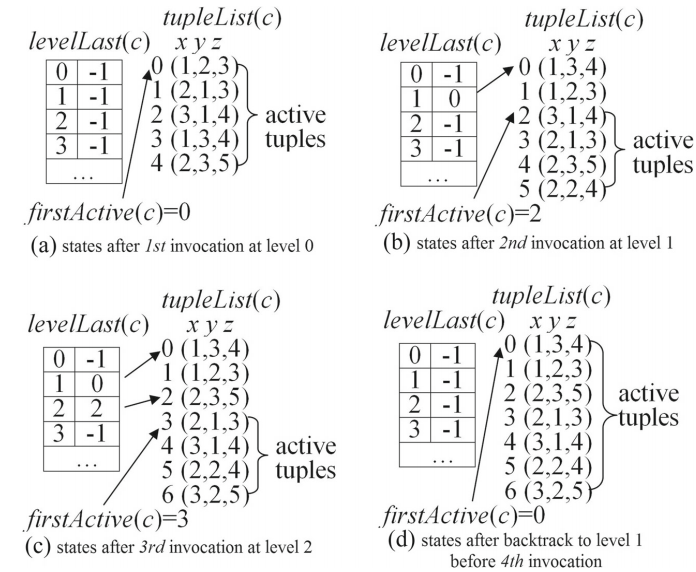
\includegraphics[width=50cm,height=10cm,keepaspectratio]{GTR.png}
	\caption{Data Structures of GTR algorithm}
	\label{fig:data_structures}
\end{figure*}

\noindent When the algorithm $ GTR $ is at level $ p $ then all the tuples of $ tupleList(c) $ before $ activeLast(c) $  are verified to be invalid in previous level. For each level, all the tuples with residue supports are identified in the first part of the algorithm and in the second part the residue supports for rest of the values are found. If a value from a variable's domain is removed by other constraint then the tuples of the indices from $ levelLast(c).size()-1 $ to $ firstActive(c) $ are checked to find the invalid tuples and the $ firstActive(c) $ and $ leveLast(c) $ are updated. Since the algorithm checks only the tuples up to $firstActive(c)$ so repeated tuple checking is avoided. If the search backtracks, then $ firstActive(c) $ can be updated using the array $ levelLast(c)$.\\
 Suppose, we have a constraint $ c: x = y + z $ involving three variables $ x,y,z $ where the domains of x,y and z are $ D_{x} = D_{y} = \{1,2,3\} $ and $ D_{z} =  \{3,4,5\}$
 
\textbf{(a)} At the $ 0^{th} $ label the algorithm finds supports for all values of each variables domain and the tuples are added to the $ tupleList(c) $. Since all the tuples are yet to be tested so $ firstActive(c) $ = 0 [Figure \ref{fig:data_structures}(a)]

\textbf{(b)} Suppose, (x,1) is removed by other constraint at level 1 so index 4 to 0 of $ tupleList(c) $ are checked and tuples (1,2,3) and (1,3,4) are removed. Therefore, $firstActive(c) $ = 2 and $ levelLast(c)[1] = $ 0. For (y,2) the algorithm finds a new support (2,2,4) in part 2. Hence, (2,2,4) is added to the end of the tuple list.

\textbf{(c)} Let, (y,3) is removed by another constraint. So the algorithm checks from index 5 to index 2 at level 2. (2,3,5) is removed from the list. Now, $ firstActive(c) = $ 3 and $ levelLast(c) = $ 2.   (3,2,5) is found as a new support for (z,5) and added to the end of the $ tupleList(c).$

\textbf{(d)} If the constraint c is never checked again and the search backtracks to level 1, then both (x,1) and (y,3) are restored. Besides, $ firstActive(c) $ is restored as 0 and $ levelLast(c)[2]$ and $levelLast(c)[1] $ are set to -1.
\section{Results}
\noindent The constraints on which the proposed method are implemented are tight non-binary constraints. For simplicity I have implemented the method for randomly generated binary-constraints and compared with other algorithms like AC1,AC2,AC3 and AC4. GTR algorithm performs as good as other algorithms in terms of running time and also pass the Anova's test with hsd tuckey.\begin{table}[!ht]
	\fontsize{8}{10} \selectfont
	\begin{tabular}{|L{2cm}|L{1.4cm}|L{1.7cm}|L{1.5cm}|}\hline
		\centering
		Treatment pairs & Tukey HSD Q statistic &  Tukey HSD p-value & Tukey HSD 
		inferfence\\ \hline
		\centering	AC3 vs AC3GTR & \centering 2.8209 & 0.0468329 & * p \textless  0.05\\ \hline
	\end{tabular}
\vspace*{0.1em}
	\caption*{TABLE 1: Anova's Test with hsd tuckey result}
	\label{tab:tuckey_test_result}
\end{table}\newpage
	





%\section{Positive Aspects}
%Positive Aspects
%\section{Limitations}
%Limitations
%\section{Conclusion}
%Conclusion

	\begin{minipage}{\textwidth}
		\begin{minipage}[b]{0.49\textwidth}
			\centering
	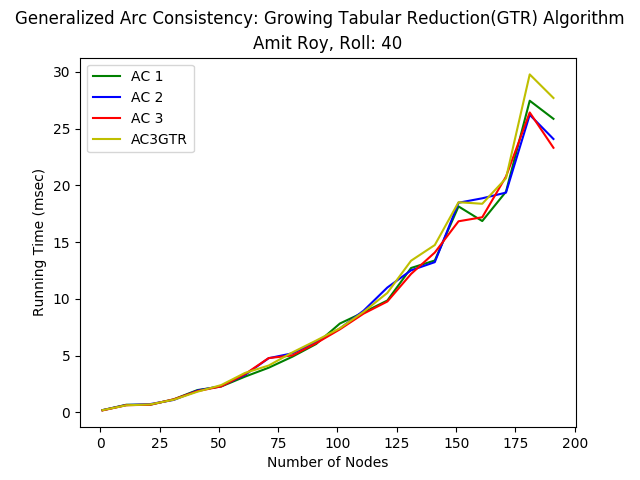
\includegraphics[width=7cm]{performance.png}
			\captionof{figure}{Running time vs number of nodes (1\texttildelow200)}
		\end{minipage}
		\hfill
		\begin{minipage}[b]{0.5\textwidth}
			\centering
			\begin{tabular}{|l|l|l|l|}
				\hline
				Treatment $\to$ & AC3& AC3GTR& Pooled Total \\ \hline
				observations N& 180& 180& 360\\ \hline
				sum $\sum$ \textit{x$ _{i} $}& 196.6006  & 204.1778& 400.7784\\ \hline
				mean $\overline{x}$  & 1.0922&1.1343&1.1133\\ \hline
				sum of squares $\sum$ \textit{x$ _{i} ^{2} $}&221.7041 & 238.9809	&460.6851\\ \hline
				sample variance \textit{s$^{2} $} & 0.0389&0.0412& 0.0404\\ \hline
				sample std. dev. \textit{s}&0.1974&0.2030&0.2010\\ \hline
				std. dev. of mean \textit{SE$ _{\overline{x}}$}& 
				0.0147	&0.0151&0.0106\\ \hline
			\end{tabular}
			\vspace*{1em}
			\captionsetup{singlelinecheck = false, format= hang,  font=footnotesize, labelsep=space}
			\captionof{table}{Descriptive statistics of k=4 independent treatments}
%			\caption{Descriptive statistics of k=4 independent treatments}
		\end{minipage}
	\end{minipage}\\\\
\section{Conclusion}
The worst-case time complexity of GTR to
establish GAC at the preprocessing step is $ O(er^{3}d^{r+1}) $ with
space complexity $ O(er^{2}d) $.
The experiment is performed on binary-constraint but it is more suitable for non-binary tight constraints because GTR algorithm has more improvement in non-binary constraints than in binary constraints. But still this algorithm performs as good as AC algorithms for binary constraints and avoids repeated constraints.
\end{document}